\chapter{Meilensteine und Zeitplan}
\label{kap:meilensteine_zeitplan}
Die Meilensteine wurden aufgrund des beschriebenen Vorgehens in Kapitel \ref{kap:forschungsdesign} definiert. Der Hauptteil der Masterarbeit besteht in der Implementierung eines Visual Analytic Tools. Anschliessend sollen Trends und Anomalien im Zugnetzwerk der \acrshort{sbb} mithilfe des entwickelten Tools exploriert werden. Für die Entwicklung sind die Meilensteine M0 bis M2 vorgesehen. Wie bereits in Kapitel \ref{kap:forschungsdesign} erwähnt, wird das VA-Tool als Web-Applikation (Frontend, Backend und \acrshort{rest}-Schnittstelle) umgesetzt. Das Explorieren der Daten mithilfe des Tools erfolgt im Meilenstein M3. Dem Autor ist es zudem wichtig, ein skalierbares VA-Tool zu entwickeln. Dies wird mithilfe des Meilensteins M4 sichergestellt (siehe Tabelle \ref{table:meilensteine}). Eine detaillierte Beschreibung zu den einzelnen Aufgaben pro Meilenstein kann der Abbildung \ref{fig_zeitplan} entnommen werden.

\begin{table}[ht]
    \caption{Übersicht der Meilensteine}
    \begin{tabularx}{\textwidth} {
        >{\raggedright\arraybackslash}X 
        >{\raggedright\arraybackslash}X}
            \hline
            \textbf{Meilenstein} & \textbf{Datum} \\
            \hline
            M0: Datenvorverarbeitung     & 18.05.2025     \\
            M1: Implementierung Frontend & 15.06.2025     \\
            M2: Implementierung Backend  & 15.06.2025     \\
            M3: Anwendung VA-Tool        & 29.06.2025     \\
            M4: Performance Analyse      & 13.07.2025     \\
            M5: Abschluss Masterarbeit   & 25.07.2025     \\
            \hline
    \end{tabularx}
    \bigbreak
    \label{table:meilensteine}
\end{table}

\begin{figure}[H]
    \caption{Zeitplan Masterarbeit (eigene Darstellung)}
    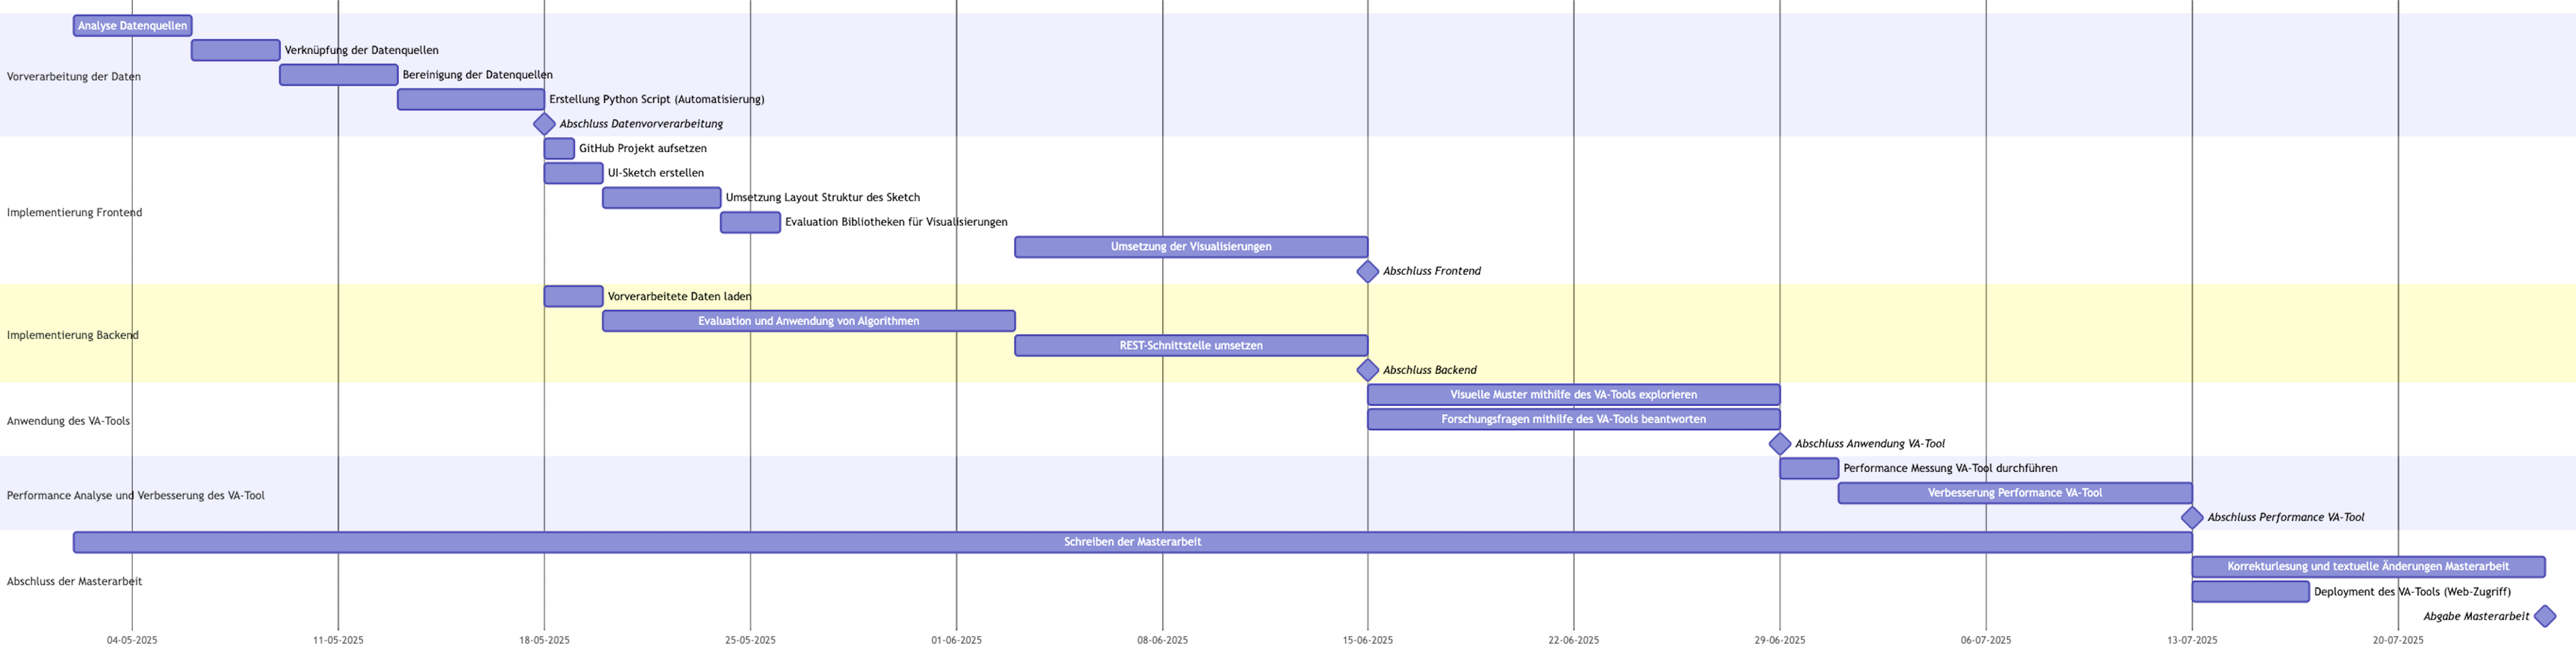
\includegraphics[width=1.0\linewidth]{content/00_assets/zeitplan.png}
    \label{fig_zeitplan}
\end{figure}



